\documentclass[uplatex,a4j]{jsreport}
\usepackage{thesis}

\begin{document}
\chapter{準備}
\label{準備}
% 読んでもらうことに必要なこと
% 自然言語処理のこと,必要な言葉
%html5のtokenizer仕様のことは3章
\section{品詞タグ}
品詞タグの説明~\cite{pennTreebankTags}
S : 節
VP : 動詞句
NP : 名詞句
VB : 動詞
NN : 名詞

\section{自然言語処理}
\subsection{使用ライブラリ}
自然言語処理のライブラリとして,Stanford CoreNLP~\cite{manning-EtAl:2014:P14-5}を使用した.
Stanford CoreNLPは自然言語処理ツールのひとつであり,スタンフォード大学によって提供されている.
StanfordCoreNLPでは,
% ライブラリでどういう情報を得られるか
形態素解析(品詞タグ付け、単語の原型の取得),構文解析,意味解析などが出来る.\\
%以下の例で詳しく述べる.\\
% pipelineの説明をする===
(pipelineの説明をする)\\
%====
\subsection{概要}
``Mika likes her dog's name.''をStanford CoreNLPで自然言語処理をさせる.
\subsubsection{トークン分割、品詞タグ付け、原型}
Mika/NNP  likes/VBZ her/PRP\$ dog/NN 's/POS name/NN ./.\\
Mika/Mika  likes/like her/she dog/dog 's/'s name/name ./.
\subsubsection{固有表現抽出}
数字や時間、アドレス、人間、地名といった固有な表現を抽出することが出来る.\\
Mika : PERSON
\subsubsection{構文木解析}
\Tree [.S [.NP [.NNP Mika ] ]
           [.VP
              [.VBZ likes ]
              [.NP [.NP [.PRP\$ her ][.NN dog ][.POS 's ] ]
                    [.NN name ] ]
           ]
           [.. . ]
      ]
\subsubsection{係り受け解析}
係り受け解析とは、単語間の関係を解析するものである.\\
\begin{figure}[h]
  \centering
  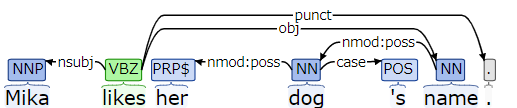
\includegraphics[keepaspectratio, scale=1.0]
       {figure/dependency.png}
  \caption{dependency(仮)}
  \label{dependency}
\end{figure}
\subsubsection{参照関係の解析}
参照関係の解析とは,文章内で複数個同じものを指し示す単語がある時、それを抽出するものである.itやheなどの指示語の指し示すものを見つける時になどに使用される.\\
Mika, her
\end{document}